\documentclass[a4paper, 12pt]{article}

%Ukrainian language

\usepackage[T1,T2A]{fontenc}
\usepackage[utf8]{inputenc}
\usepackage[english,ukrainian]{babel}
\usepackage{indentfirst}

%Listings
\usepackage{listings}
\usepackage{xcolor}

%New colors defined below
\definecolor{codegreen}{rgb}{0,0.6,0}
\definecolor{codegray}{rgb}{0.5,0.5,0.5}
\definecolor{codepurple}{rgb}{0.58,0,0.82}
\definecolor{backcolour}{rgb}{0.97,0.97,0.97}

%Code listing style named "mystyle"
\lstdefinestyle{mystyle}{
  backgroundcolor=\color{backcolour},   commentstyle=\color{codegreen},
  keywordstyle=\color{magenta},
  numberstyle=\tiny\color{codegray},
  stringstyle=\color{codepurple},
  basicstyle=\ttfamily\footnotesize,
  breakatwhitespace=false,         
  breaklines=true,                 
  captionpos=b,                    
  keepspaces=true,                 
  numbers=left,                    
  numbersep=5pt,                  
  showspaces=false,                
  showstringspaces=false,
  showtabs=false,                  
  tabsize=2
}

\lstset{style=mystyle}

%Verbatim
\usepackage{fancyvrb}
\usepackage{upquote,textcomp}

%Math
\usepackage{amsmath,amsfonts,amssymb,amsthm,mathtools} 

% Images
\usepackage{graphicx}
\usepackage{wrapfig}

%Vector graphics
\usepackage{tikz}
\usetikzlibrary{positioning}
\usetikzlibrary{patterns}

%Plots
\usepackage{pgfplots}
\pgfplotsset{compat=1.9}

%Title
\author{Демедюк Віталій}
\title{Звіт лабораторного практикуму\\
       з інформаційних технологій\\
       "Фрагментарна реалізація систем управління табличними базами даних"\\
       Варіант - "16"}
%\date{\today}

%Text color
\usepackage{xcolor}

%Multirow
\usepackage{multirow}

\usepackage{float}

\usepackage{bigstrut}
\usepackage{colortbl}

\usepackage[pdftex,
colorlinks,%
linkcolor=blue,citecolor=red,urlcolor=blue,
hyperindex,%
plainpages=false,%
bookmarksopen,%
bookmarksnumbered,%
unicode]{hyperref}

\begin{document}

\maketitle

\newpage

\tableofcontents

\newpage

\section{Постановка задачі}

\textbf{Вимоги щодо структури бази:}

\begin{itemize}
\item кількість таблиць принципово не обмежена (реляції між таблицями не враховувати);
\item кількість полів та кількість записів у кожній таблиці також принципово не обмежені.
\end{itemize}


\textbf{У роботі треба забезпечити підтримку (для полів у таблицях) наступних типів:}

\begin{itemize}
\item integer;
\item real;
\item char;
\item string;
\item текстові файли;
\item iнтервальний integer.
\end{itemize}

\textbf{Також у роботі треба реалізувати функціональну підтримку для:}

\begin{itemize}
\item створення бази;
\item створення (із валідацією даних) та знищення таблиці з бази;
перегляду та редагування рядків таблиці;
\item збереження табличної бази на диску та, навпаки, зчитування її з диску;
\item прямий добуток двох таблиць.
\end{itemize}

\section{Етап №0(попередній етап)}

\textbf{Функціональна специфікація} системи управління табличними базами даних (СУТБД) у вигляді діаграм прецедентів UML.

\begin{figure}[H]
\centering
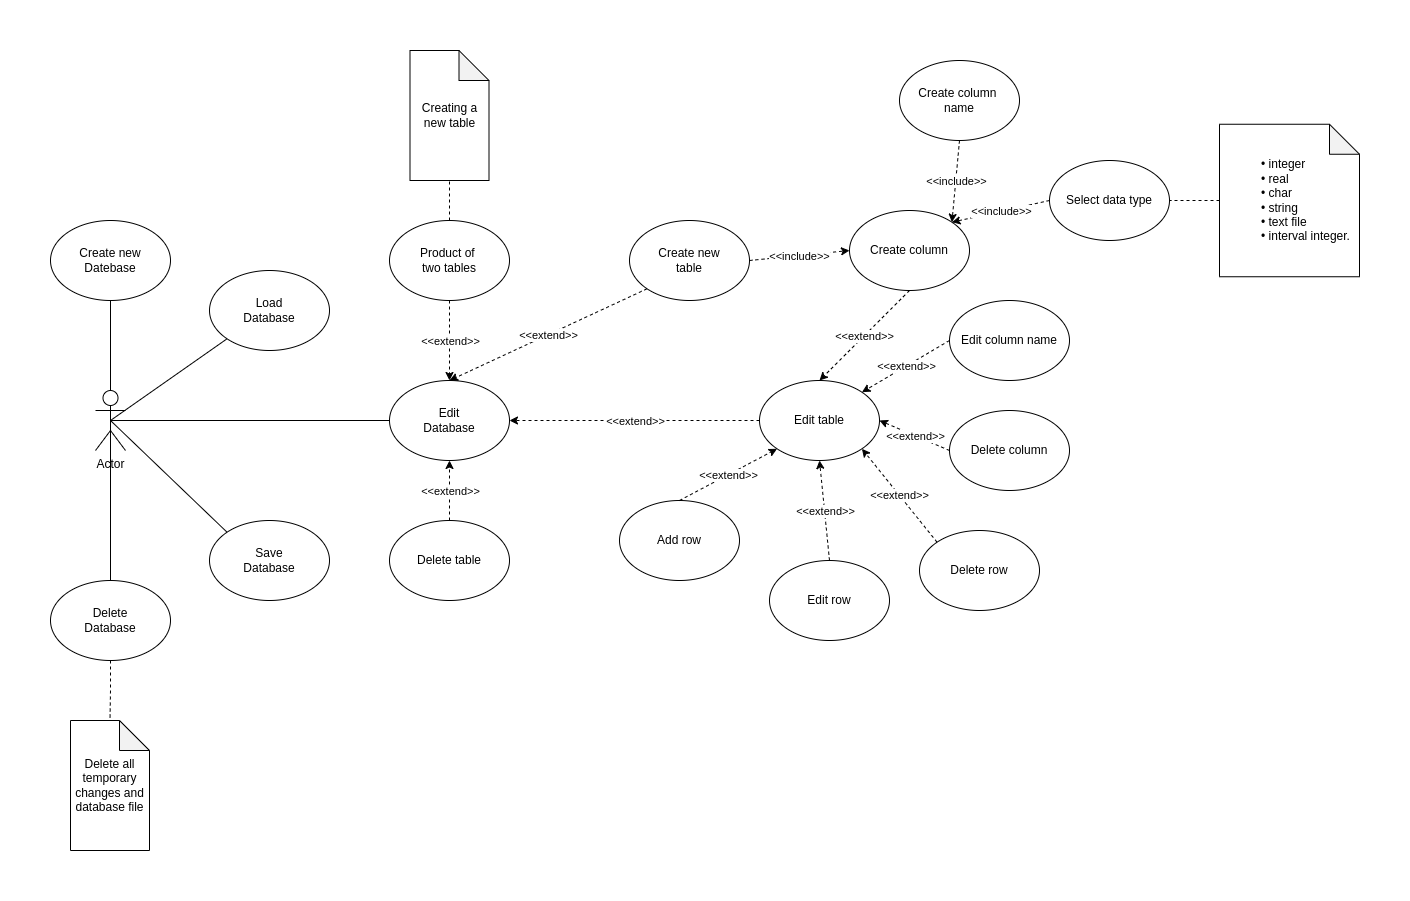
\includegraphics[scale=0.4]{../diagrams/use_case.png}
\caption{Інтерфейс на основі форм:}
\end{figure}

\section{Етап №1}
Розробка власних класів для понять "Таблиця", "База" та, можливо, деяких інших класів, спряжених із поняттям "Таблиця" (наприклад, "Схема таблиці", "Атрибут", "Рядок таблиці" тощо). Створення UML-діаграми класів (з наявними між класами відношеннями).

\begin{figure}[H]
\centering
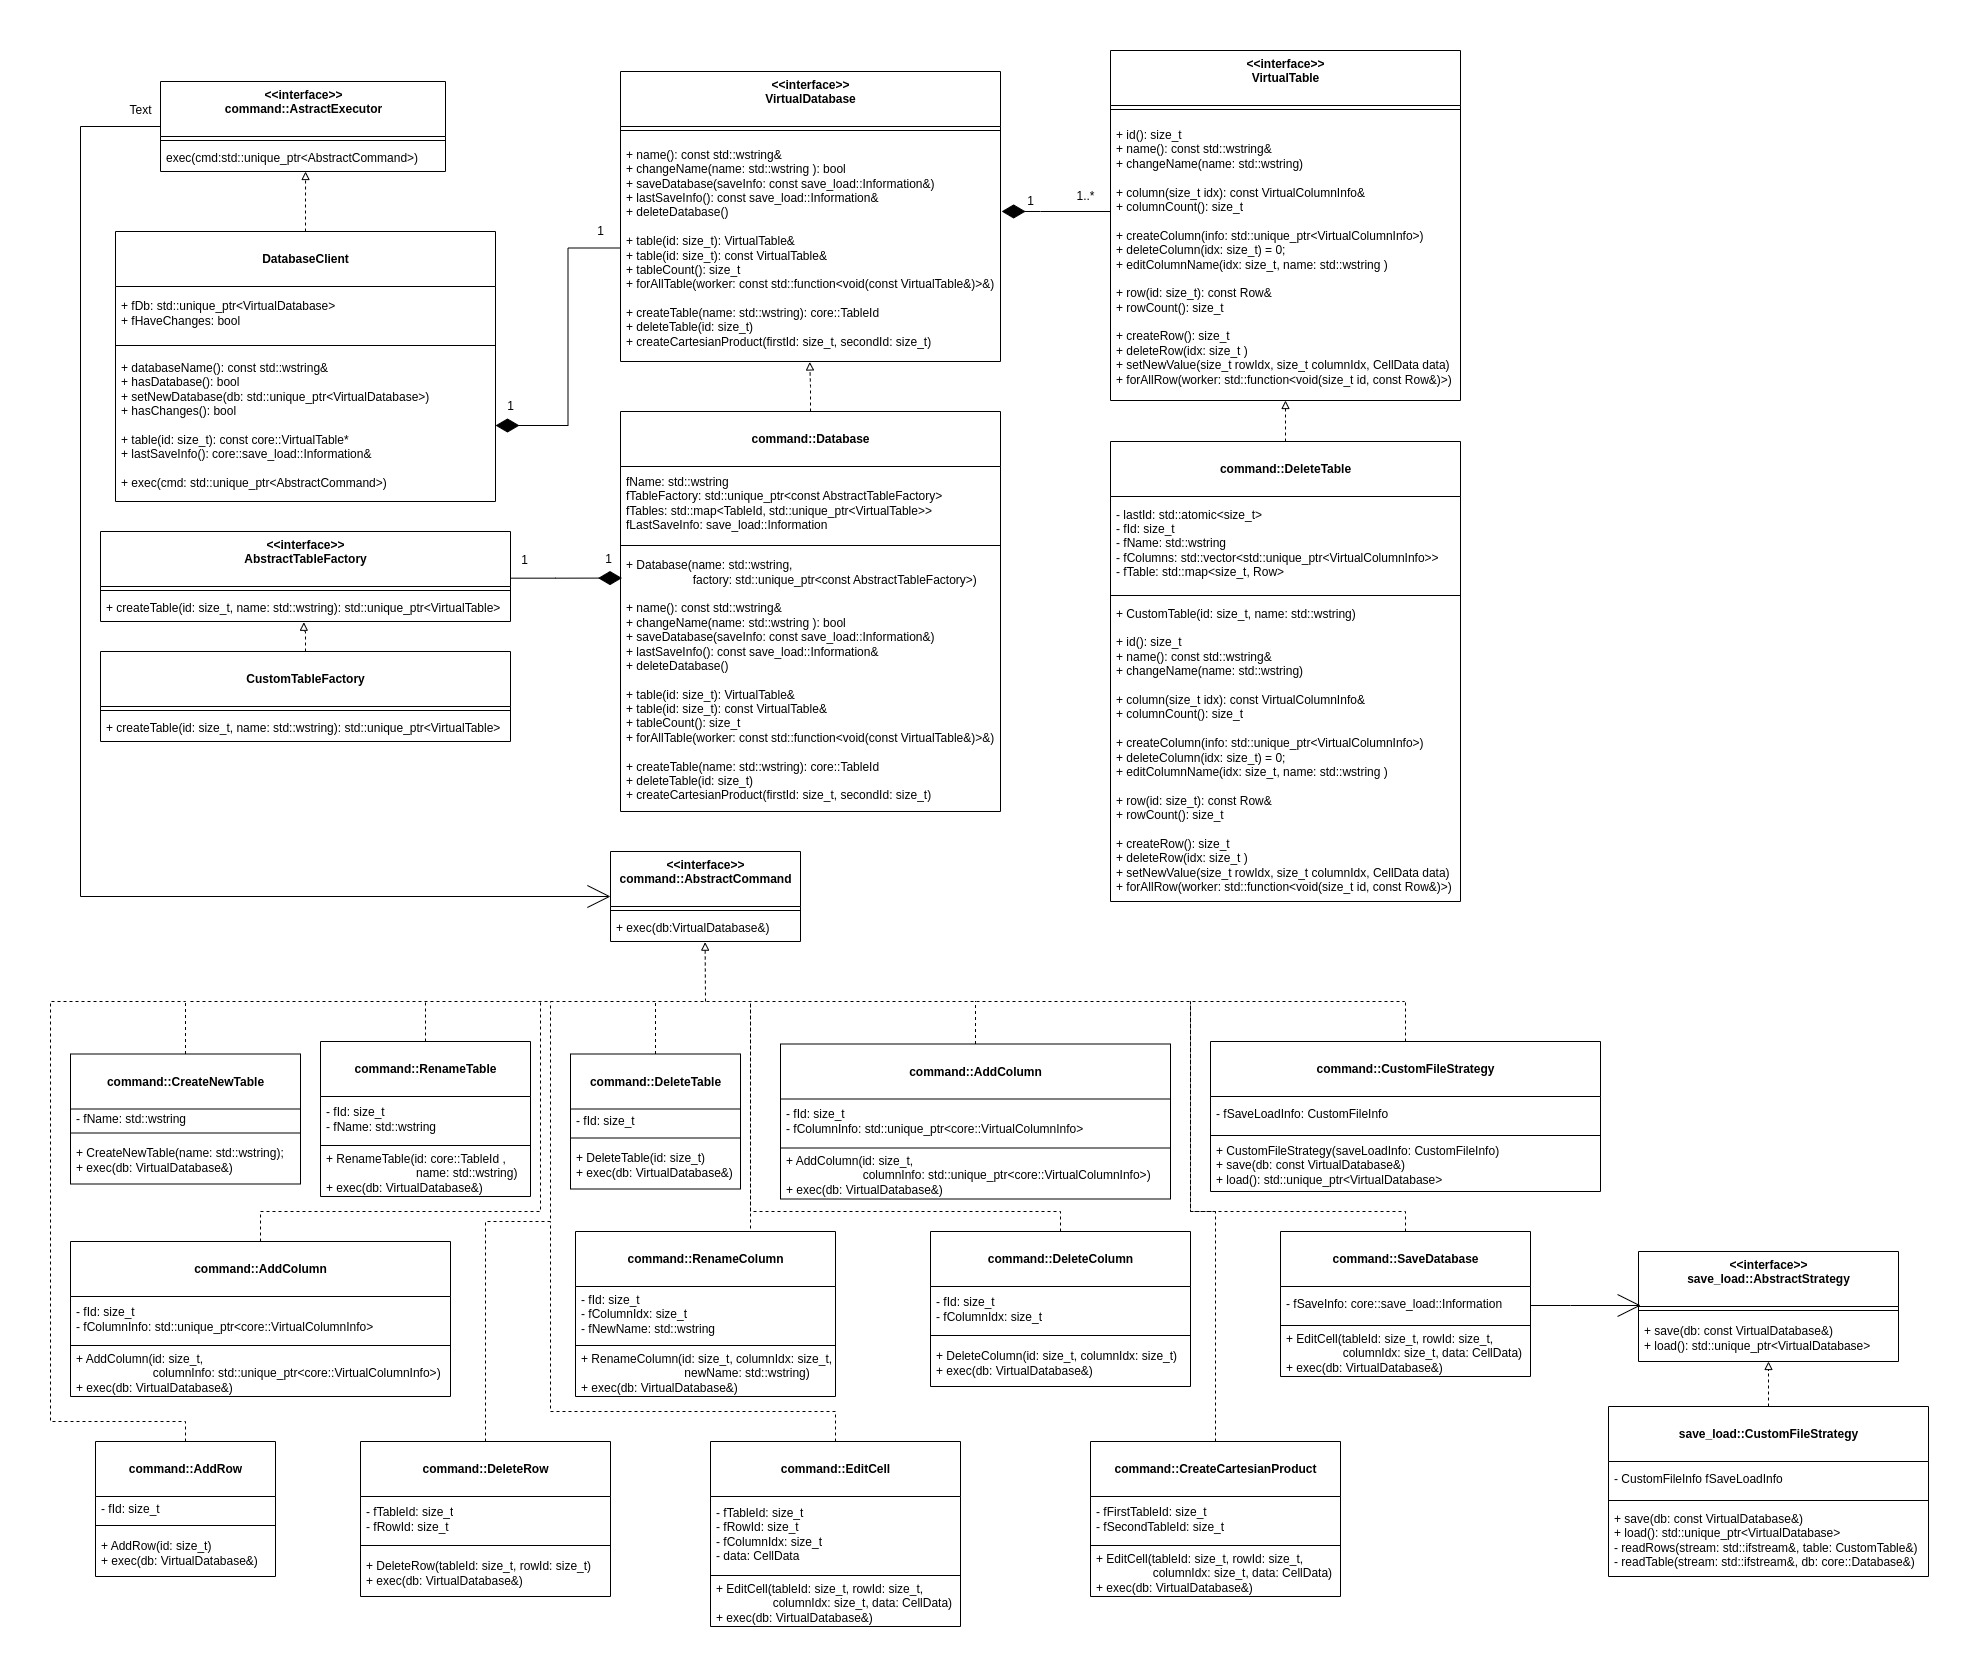
\includegraphics[scale=0.3]{../diagrams/IT_UML_DIAGRAM.png}
\caption{Діаграма прицедентів}
\end{figure}

\section{Етап №2}
Проведення unit-тестування та забезпечення інтерфейсу користувача на основі форм

\begin{figure}[H]
\centering
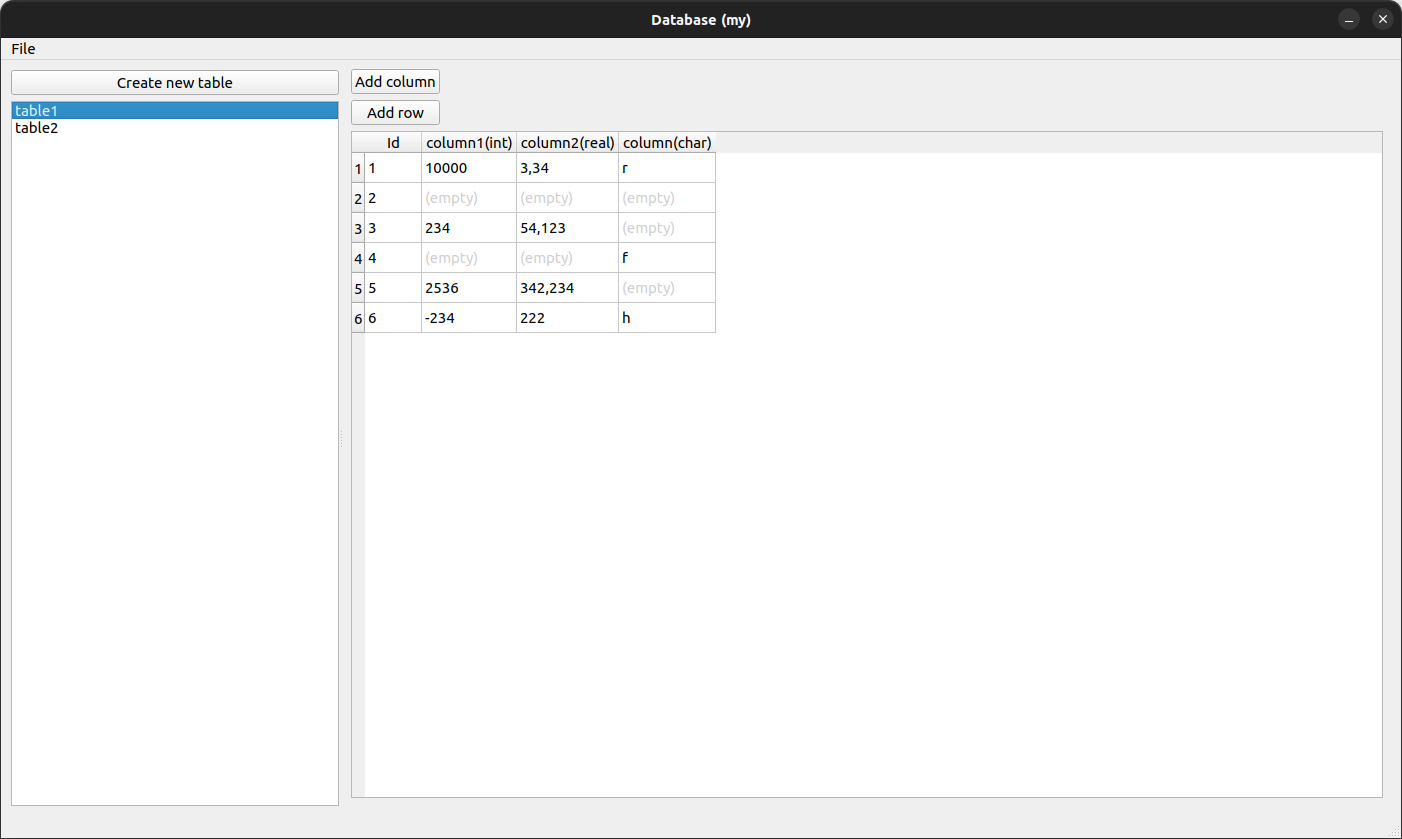
\includegraphics[scale=0.3]{resources/DesktopWindow.png}
\caption{UML діаграма класів}
\end{figure}

\begin{figure}[H]
\centering
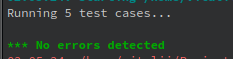
\includegraphics[scale=0.8]{resources/UnitTests.png}
\caption{Результат виконання unit-тестів}
\end{figure}

\section{Етап №3}
Використання реляційної СУБД(SQLite) для серіалізації об'єктів для збереження даних.
 
\begin{figure}[H]
\centering
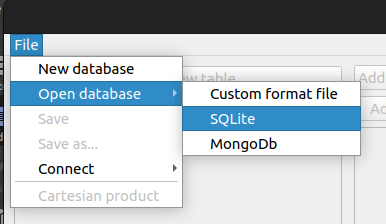
\includegraphics[scale=0.8]{resources/SQLiteLoadMenu.png}
\caption{Стільниковий клієнт. Завантаження даних з SQLite}
\end{figure} 

\begin{figure}[H]
\centering
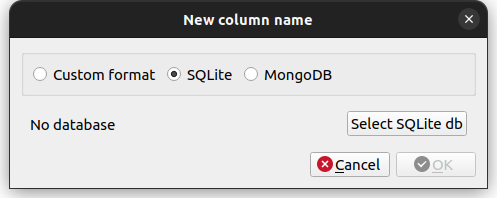
\includegraphics[scale=0.8]{resources/SQLiteSaveDialog.png}
\caption{Діалог збереження в SQLite}
\end{figure} 

\begin{figure}[H]
\centering
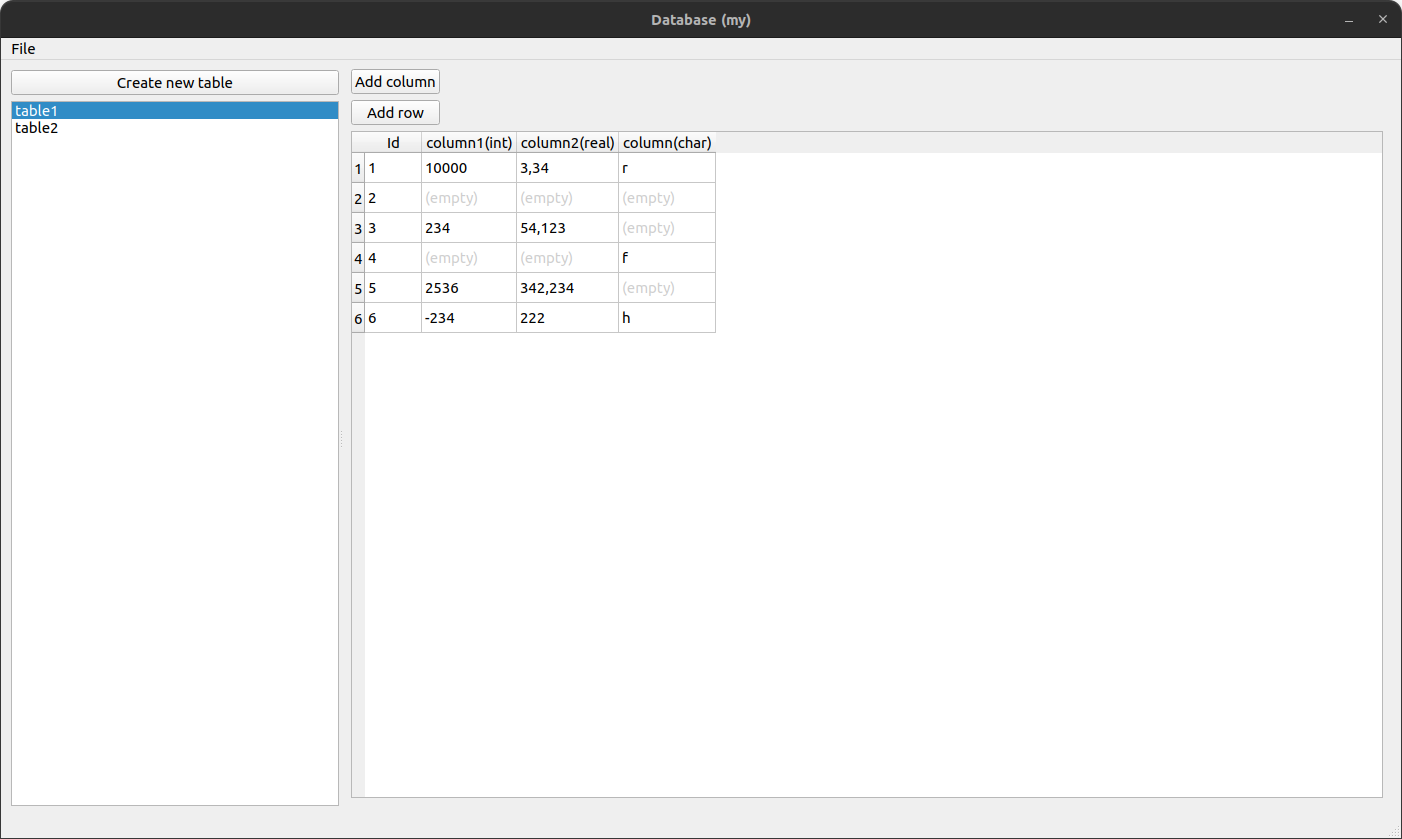
\includegraphics[scale=0.3]{resources/SQLite.png}
\caption{SQLite база даних після збереження}
\end{figure} 
 
\section{Етап №4}
Використання  СУБД Mongo для серіалізації об'єктів для збереження даних.

\begin{figure}[H]
\centering
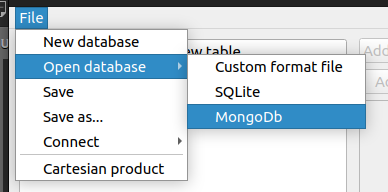
\includegraphics[scale=0.8]{resources/MongoDbLoadMenu.png}
\caption{Стільниковий клієнт. Завантаження даних з MongoDb}
\end{figure} 

\begin{figure}[H]
\centering
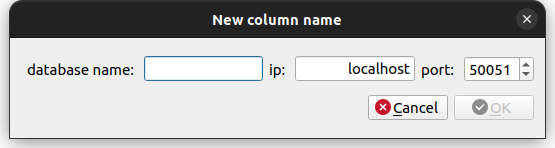
\includegraphics[scale=0.8]{resources/MongoDbLoadDialog.png}
\caption{Діалог завантаження з MongoDb}
\end{figure} 

\begin{figure}[H]
\centering
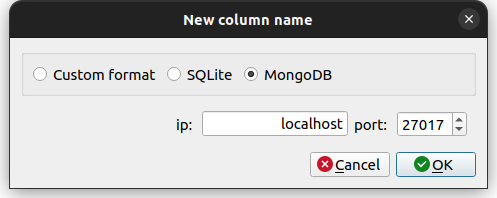
\includegraphics[scale=0.8]{resources/MongoDbSaveDialog.png}
\caption{Діалог збереження в MongoDb}
\end{figure} 

\begin{figure}[H]
\centering
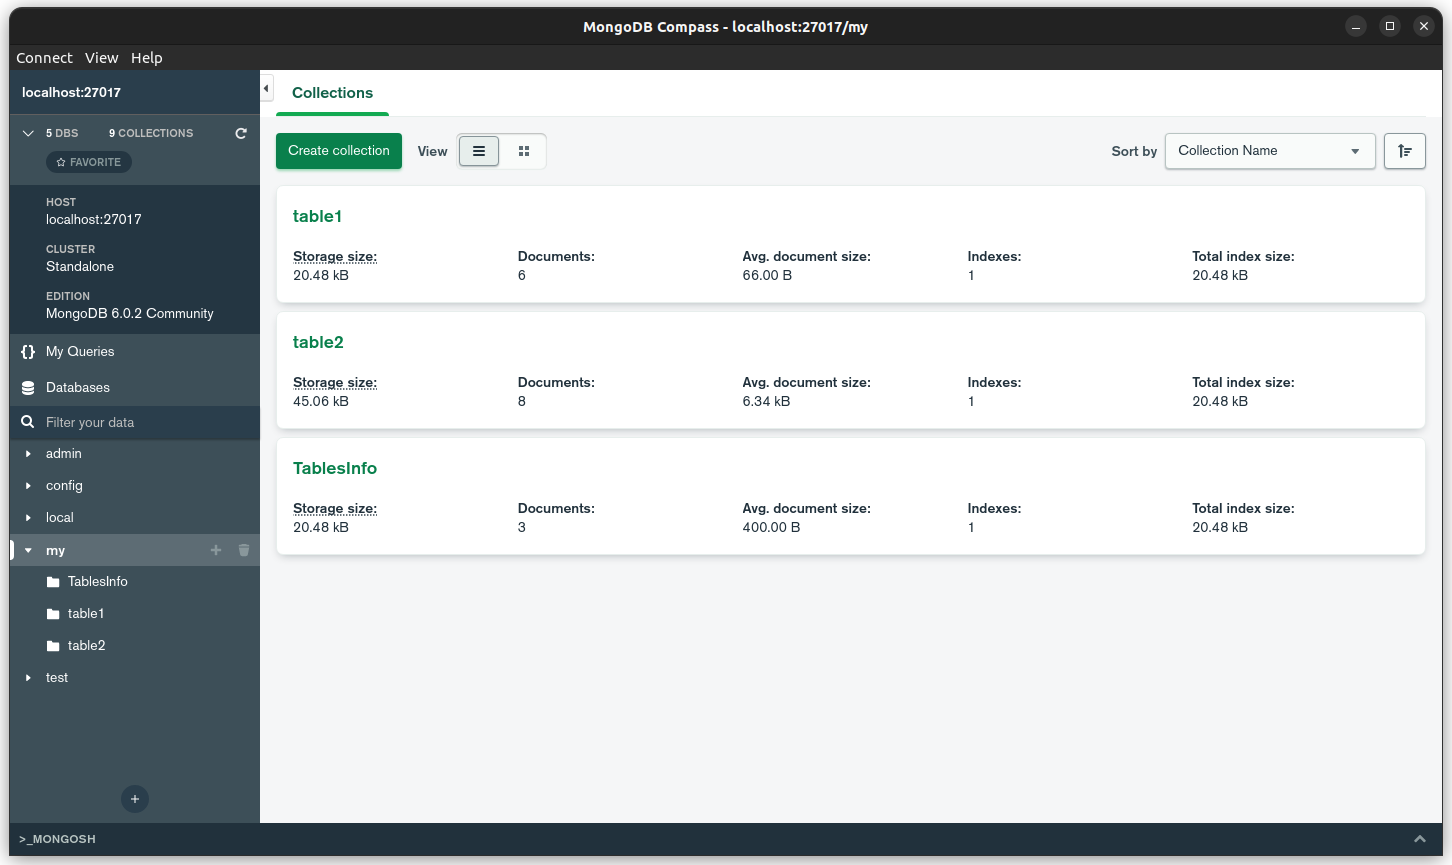
\includegraphics[scale=0.3]{resources/MongoDb.png}
\caption{MongoDb база даних після збереження}
\end{figure} 

\section{Етап №5}

Розробка gRpc клієнта і сервера на одній мові програмування.

\begin{figure}[H]
\centering
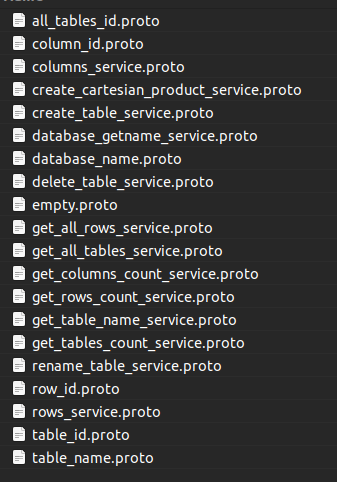
\includegraphics[scale=0.3]{resources/ProtoFiles.png}
\caption{Усі proto файли}
\end{figure}

\begin{lstlisting}[caption=код gRpc сервіса для отриманя рядка таблиці]
service RowsService {
    rpc get(RowId) returns (Row) {}
    rpc create(TableId) returns (RowCreateResponse) {}
    rpc editCell(CellEditRequest) returns (Empty) {}
    rpc deleteRow(RowId) returns (Empty) {}
}
\end{lstlisting}

\begin{figure}[H]
\centering
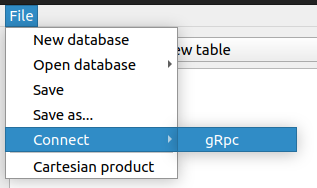
\includegraphics[scale=0.5]{resources/gRpcClientMenu.png}
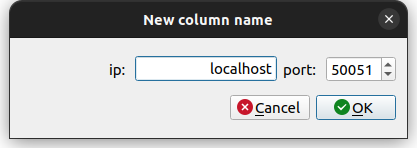
\includegraphics[scale=0.5]{resources/gRpcClientDialog.png}
\caption{Інтерфейс стільникового кліжента для підключення до сервера}
\end{figure}

\begin{figure}[H]
\centering
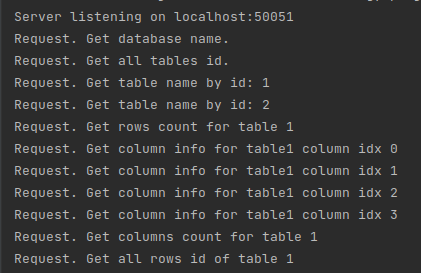
\includegraphics[scale=0.5]{resources/gRpcServerLogs.png}
\caption{Фрагмент логів gRpc сервера}
\end{figure}

\section{Етап №6-7}
У цьому етапі був розроблений gRpc клієнт на мові Python для сервера, який був розроблений в етапі №5. Одночасно цей клієнт є GraphQL сервером.

\begin{figure}[H]
\centering
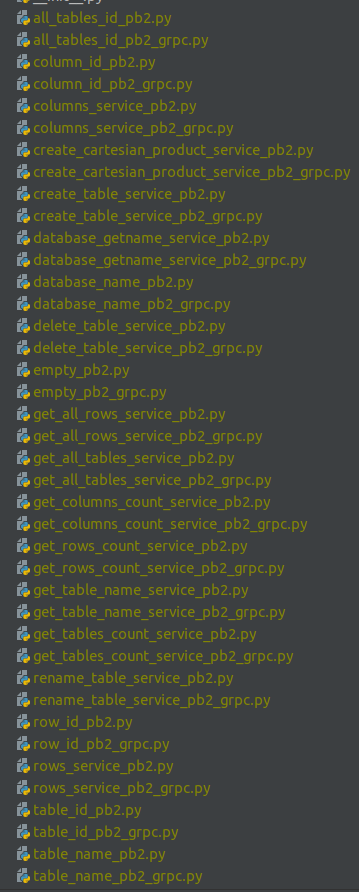
\includegraphics[scale=0.5]{resources/gRpcPythonFiles.png}
\caption{Згенеровані proto/grpc файли для Python клієнта}
\end{figure}

\begin{lstlisting}[caption=GraphQL schema]
schema {
    query: Query
    mutation: Mutation
}

type TableListItem {
    id: ID!
    name: String!
}

type GetTableListResult {
    success: Boolean!
    errors: [String!]
    tables_list: [TableListItem!]
}

type ColumnInfo {
    name: String!
    type: String!
    lower_limit: Int
    upper_limit: Int
}

type TableInfo {
    table_name: String!
    columns: [ColumnInfo!]
}

type GetTableInfoResult {
    success: Boolean!
    errors: [String!]
    table_info: TableInfo
}

type IntegerWrapper {
    int_value: Int!
}

type RealWrapper {
    real_value: Float!
}

type CharWrapper {
    char_value: String!
}

type StringWrapper {
    str_value: String
}

type File {
    filename: String!
}

type IntervalInteger {
    int_value: Int!
}

union Cell = IntegerWrapper | RealWrapper | CharWrapper | StringWrapper | File | IntervalInteger

type Row {
    row_id: Int
    cells: [Cell]
}

type Table {
    rows: [Row!]
}

type GetTableResult {
    success: Boolean!
    errors: [String!]
    table: Table
}

type Query {
    getTableList: GetTableListResult!
    getTableInfo(table_id: ID): GetTableInfoResult
    getTable(table_id: ID): GetTableResult
}

type MutationResult {
    success: Boolean!
    errors: [String!]
}

type Mutation {
    createNewTable(name: String!): MutationResult
    renameTable(table_id: Int!, new_name: String!): MutationResult!
    deleteTable(table_id: Int!): MutationResult!

    createDefaultColumn(table_id: Int!, name: String!, column_type: String!): MutationResult!
    createIntIntervalColumn(table_id: Int!, name: String!, lower_limit: Int!, upper_limit: Int!): MutationResult!
    renameColumn(table_id: Int!, column_idx: Int!, new_name: String!): MutationResult!
    deleteColumn(table_id: Int!, column_idx: Int!): MutationResult!

    createNewRow(table_id: Int!): MutationResult!
    deleteRow(table_id: Int!, row_id: Int!): MutationResult!
    editIntCell(table_id: Int!, column_idx: Int!, row_id: Int!, data: Int!): MutationResult!
    editRealCell(table_id: Int!, column_idx: Int!, row_id: Int!, data: Float!): MutationResult!
    editCharCell(table_id: Int!, column_idx: Int!, row_id: Int!, data: String!): MutationResult!
    editStringCell(table_id: Int!, column_idx: Int!, row_id: Int!, data: String!): MutationResult!
    editIntervalIntCell(table_id: Int!, column_idx: Int!, row_id: Int!, data: Int!): MutationResult!
    clearCell(table_id: Int!, column_idx: Int!, row_id: Int!): MutationResult!

    createCartesianProduct(first_table_id: Int! second_table_id: Int!): MutationResult!
}
\end{lstlisting}

\begin{figure}[H]
\centering
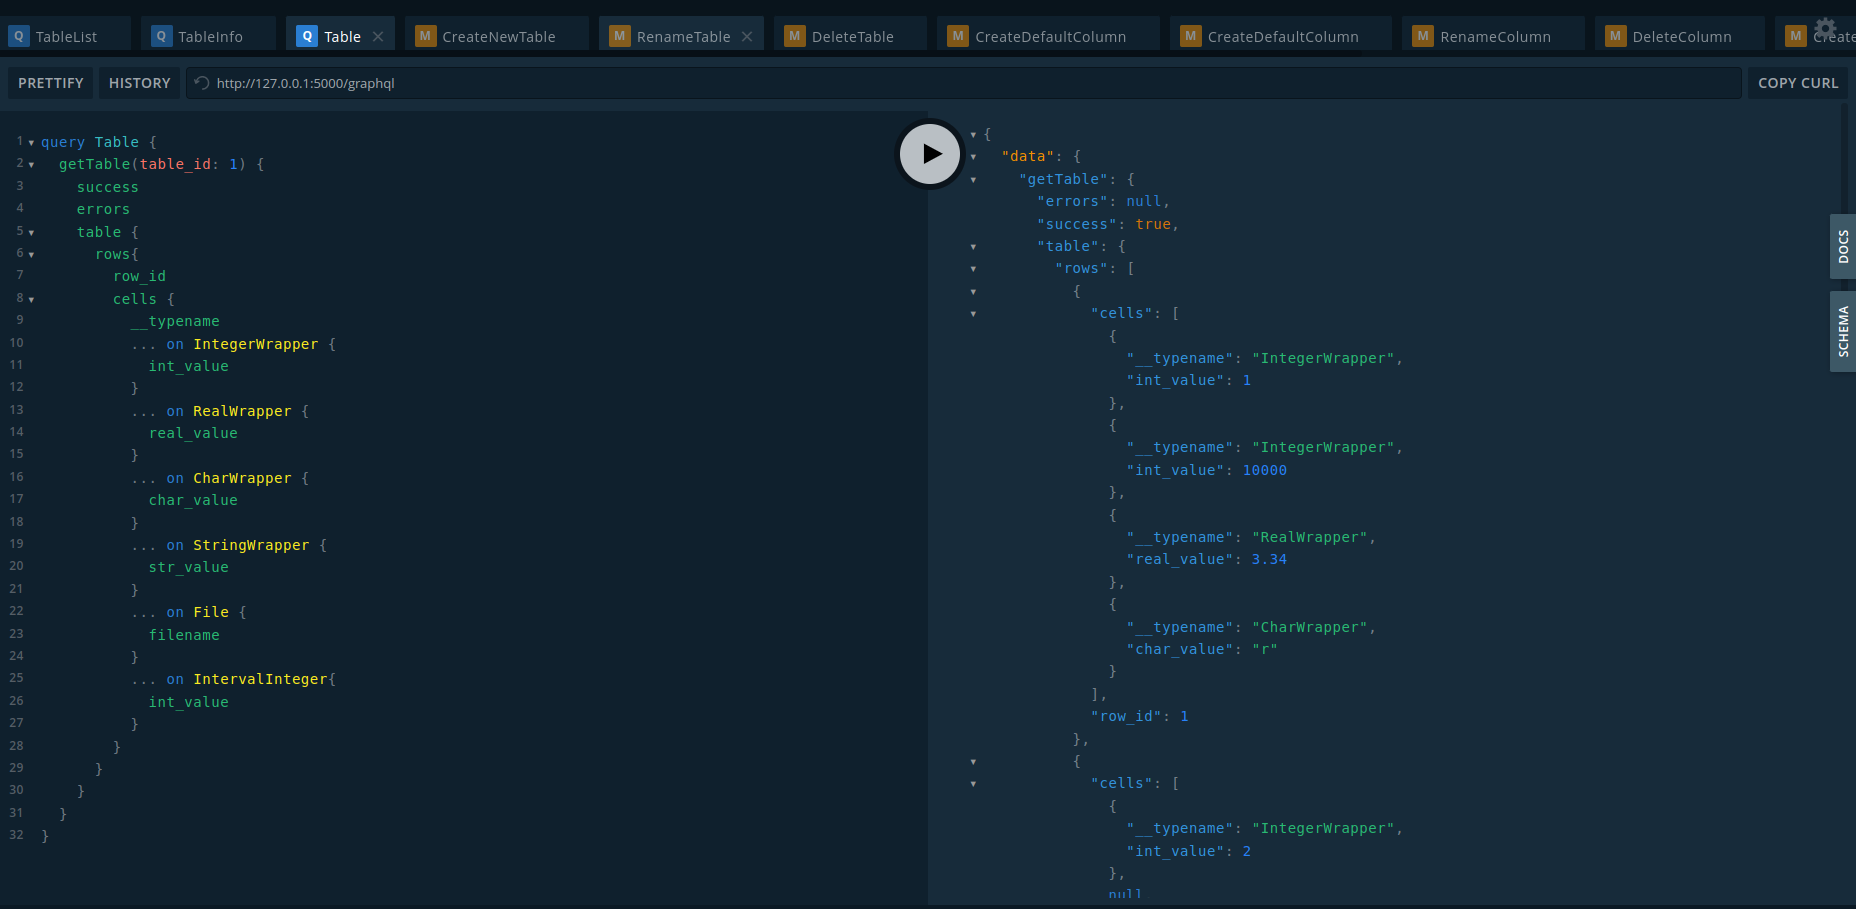
\includegraphics[scale=0.32]{resources/GraphQLTableQuery.png}
\caption{GraphQL. Запит на отримання всієї таблиці}
\end{figure}

\section{Етап №8}

Розгортання gRpc сервера з 5-го етапу.

\begin{lstlisting}[caption=фрагмент Dockerfile для деплою сервера]
ENTRYPOINT export LD_LIBRARY_PATH=/usr/local/lib \
           && ./build/gRpcDatabaseServer --load-type="custom" --database-file="../custom_test_db_projects/my.cdb" --server-ip="0.0.0.0" --server-port="50051"
\end{lstlisting}

\begin{figure}[H]
\centering
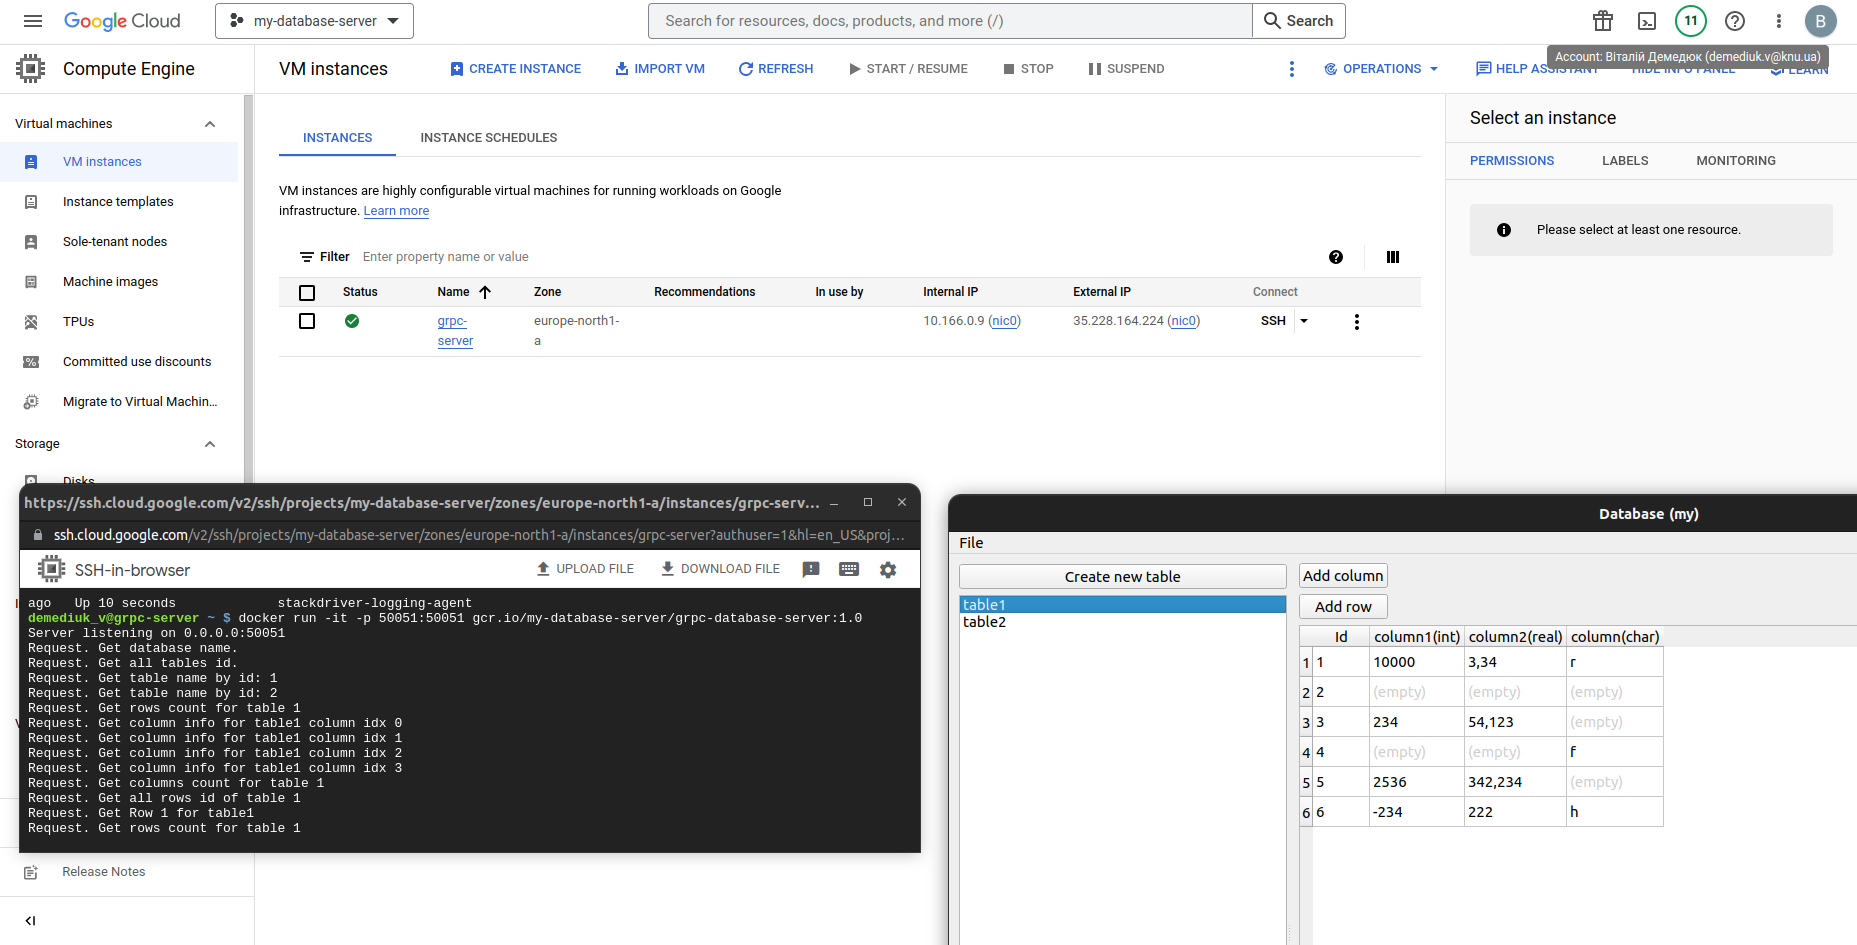
\includegraphics[scale=0.32]{resources/Cloud.png}
\caption{Cloud Google Platform}
\end{figure}

\end{document}